We start from the 'bare-bones' heat transport equation (source terms are omitted): 
\begin{equation}
\rho C_p \left( \frac{\partial T}{\partial t} + {\vec \upnu}\cdot {\vec\nabla T} \right)
= {\vec \nabla} \cdot \left( k \vec\nabla T \right)
\end{equation}
In what follows we assume that the velocity vield $\vec \upnu$ is known so that temperature is the 
only unknown.
Let $N^\uptheta$ be the temperature basis functions so that the temperature inside an element is 
given by\footnote{the $\uptheta$ superscript has been chosen to denote temperature so as to avoid confusion
with the transpose operator}:
\begin{equation}
T^h({\vec r}) = \sum_{i=1}^{m_T} N^\uptheta_i ({\vec r}) T_i = \vec N^\uptheta \cdot \vec T
\end{equation}
where $\vec T$ is a vector of length $m_T$
The weak form is then 
\begin{equation}
\int_\Omega N^\uptheta_i \left[ 
\rho C_p \left( \frac{\partial T}{\partial t} + {\vec \upnu}\cdot {\vec\nabla T} \right) \right] d\Omega
= \int_\Omega  N^\uptheta_i {\vec \nabla} \cdot k \vec\nabla T  d\Omega
\end{equation}

\[
\underbrace{\int_\Omega N^\uptheta_i  \rho C_p \frac{\partial T}{\partial t} d\Omega}_{I}
+ \underbrace{\int_\Omega N^\uptheta_i  \rho C_p  {\vec \upnu}\cdot {\vec\nabla T}   d\Omega}_{II}
= \underbrace{\int_\Omega  N^\uptheta_i {\vec \nabla} \cdot k \vec\nabla T d\Omega}_{III}
\quad\quad
i=1,m_T
\]

Looking at the first term:
\begin{eqnarray}
\int_\Omega N^\uptheta_i  \rho C_p \frac{\partial T}{\partial t} d\Omega
&=&  \int_\Omega N^\uptheta_i  \rho C_p \vec N^\uptheta \cdot \dot{\vec T}  d\Omega \\
\end{eqnarray}
so that when we assemble all contributions for $i=1,m_T$ we get:
\[
I 
= \int_\Omega \vec N^\uptheta  \rho C_p \vec N^\uptheta \cdot \dot{\vec T}  d\Omega
= \left( \int_\Omega \rho C_p  \vec N^\uptheta  \vec N^\uptheta  d\Omega \right) \cdot \dot{\vec T}
= {\bm M}^T \cdot \dot{\vec T}
 \]
where ${\bm M}^T$ is the mass matrix of the system of size $(m_T \times m_T)$ with 
\[
M_{ij}^T = \int_\Omega \rho C_p N_i^\uptheta N_j^\uptheta d\Omega
\]
Turning now to the second term:
\begin{eqnarray}
\int_\Omega N^\uptheta_i  \rho C_p  {\vec \upnu}\cdot {\vec\nabla T}   d\Omega
&=& \int_\Omega N^\uptheta_i  \rho C_p (u \frac{\partial T}{\partial x} +  v \frac{\partial T}{\partial y} ) d\Omega \\
&=& \int_\Omega N^\uptheta_i  \rho C_p (u \frac{\partial \vec N^\uptheta}{\partial x} +  v \frac{\partial \vec N^\uptheta}{\partial y} ) \cdot \vec T d\Omega \\
\end{eqnarray}
so that when we assemble all contributions for $i=1,m_T$ we get:
\[
II = \left(\int_\Omega \rho C_p \vec N^\uptheta (u \frac{\partial \vec N^\uptheta}{\partial x} +  v \frac{\partial \vec N^\uptheta}{\partial y} ) d\Omega \right)  \cdot \vec T = {\bm K}_a \cdot \vec T
\]
where ${\bm K}_a$ is the advection term matrix of size $(m_T \times m_T)$ with
\[
(K_a)_{ij} = \int_\Omega \rho C_p N_i^\uptheta 
\left(u \frac{\partial N_j^\uptheta}{\partial x} +  v \frac{\partial N_j^\uptheta}{\partial y} \right) d\Omega 
\]
Now looking at the third term, we carry out an integration by part and neglect the surface term for now, so that 
\begin{eqnarray}
\int_\Omega  N^\uptheta_i {\vec \nabla} \cdot k \vec\nabla T d\Omega
&=& - \int_\Omega  k \vec \nabla N^\uptheta_i \cdot \vec\nabla T d\Omega \\
&=& - \int_\Omega  k \vec \nabla N^\uptheta_i \cdot \vec\nabla (\vec N^\uptheta \cdot \vec T) d\Omega \\
\end{eqnarray}
with 
\[
\vec \nabla \vec N^\uptheta = 
\left(
\begin{array}{cccc}
\partial_x N_1^\uptheta & 
\partial_x N_2^\uptheta & \dots &
\partial_x N_{m_T}^\uptheta \\ \\
\partial_y N_1^\uptheta & 
\partial_y N_2^\uptheta & \dots &
\partial_y N_{m_T}^\uptheta 
\end{array}
\right)
\]
so that finally:
\[
III = - \left( \int_\Omega k (\vec \nabla \vec N^\uptheta)^T \cdot \vec \nabla \vec N^\uptheta d\Omega \right) \cdot \vec T
= - {\bm K}_d \cdot \vec T
\]
where ${\bm K}_d$ is the diffusion term matrix:
\[
{\bm K}_d = \int_\Omega  k (\vec \nabla \vec N^\uptheta)^T \cdot \vec \nabla \vec N^\uptheta d\Omega 
\]
 Ultimately terms $I,II,III$ together yield:
\[
\boxed{
{\bm M}^\uptheta \cdot \dot{\vec T} + ({\bm K}_a + {\bm K}_d) \cdot \vec T = \vec 0
}
\]

%What now remains to be done is to address the time derivative on the temperature vector. 
%The most simple approach would be to use an explicit Euler one, i.e.:
%\[
%\frac{\partial \vec T}{\partial t} = \frac{\vec T^{(k)} - \vec T^{(k-1)}}{\delta t}
%\]
%where $\vec T^{(k)}$ is the temperature field at time step $k$ and $\delta t$ is the time interval 
%between two consecutive time steps.
%In this case the discretised heat transport equation is:
%\[
%\boxed{
%\left( {\bm M}^\uptheta  + ({\bm K}_a + {\bm K}_d) \delta t \right) \cdot \vec T^{(k)} =  {\bm M}^\uptheta \cdot \vec T^{(k-1)}
%}
%\]
\todo[inline]{add source term!!}

%....................................................
\subsubsection{Dealing with the time discretisation} \ref{sec:timediscr}

Essentially we have to solve a PDE of the type:
\[
\frac{\partial T}{\partial t} = {\cal F}(\vec \upnu,T,\vec\nabla T,\Delta T)
\]
with ${\cal F}=\frac{1}{\rho C_p}(-\vec\upnu\cdot\vec\nabla T + \vec\nabla\cdot k\vec\nabla T)$.

\index{general}{Forward Euler}
\index{general}{Backward Euler}
\index{general}{Crank-Nicolson}

The (explicit) forward Euler method is:
\[
\frac{T^{n+1}-T^n}{\delta t} = {\cal F}^n(T,\vec\nabla T,\Delta T)
\]
The (implicit) backward Euler method is:
\[
\frac{T^{n+1}-T^n}{\delta t} = {\cal F}^{n+1}(T,\vec\nabla T,\Delta T)
\]
and the (implicit) Crank-Nicolson algorithm is:
\[
\frac{T^{n+1}-T^n}{\delta t} = 
\frac{1}{2}
\left[
{\cal F}^{n}(T,\vec\nabla T,\Delta T)
+
{\cal F}^{n+1}(T,\vec\nabla T,\Delta T)
\right]
\]
where the superscript $n$ indicates the time step.
The Crank-Nicolson is obviously based on the trapezoidal rule, with second-order convergence in time.


In what follows, I omit the superscript on the mass matrix to simplify notations: ${\bm M}^\uptheta={\bm M}$.
In terms of Finite Elements, these become:
\begin{itemize}
\item Explicit Forward euler:
\[
\frac{1}{\delta t} ({\bm M}^{n+1} \cdot \vec T^{n+1}  -{\bm M}^n \cdot \vec T^{n} )
=
-({\bm K}_a^n+{\bm K}^n_d) \cdot \vec T^{n}
\]
or, 
\[
\boxed{
{\bm M}^{n+1} \cdot \vec T^{n+1}
= \left(  {\bm M}^n  + ({\bm K}_a^n+{\bm K}_d^n) \delta t \right)\cdot \vec T^{n} 
}
\]

\item Implicit Backward euler:
\[
\frac{1}{\delta t} ({\bm M}^{n+1} \cdot \vec T^{n+1}  -{\bm M}^n \cdot \vec T^{n} )
= -({\bm K}_a^{n+1}+{\bm K}_d^{n+1}) \cdot \vec T^{n+1}
\]
or, 
\begin{equation}
\boxed{
\left( {\bm M}^{n+1} +({\bm K}_a^{n+1}+{\bm K}_d^{n+1})\delta t \right) \cdot \vec T^{n+1}
=
{\bm M}^n \cdot \vec T^{n} 
}
\label{eq:hte_ibe}
\end{equation}

\item Crank-Nicolson

\[
\frac{1}{\delta t} \left({\bm M}^{n+1} \cdot \vec T^{n+1}  -{\bm M}^n \cdot \vec T^{n} \right)
= 
\frac{1}{2}
\left[
-({\bm K}_a^{n+1}+{\bm K}_d^{n+1}) \cdot \vec T^{n+1}
-({\bm K}_a^{n}+{\bm K}_d^{n}) \cdot \vec T^{n}
\right]
\]
or,
\[
\boxed{
\left( {\bm M}^{n+1} +({\bm K}_a^{n+1}+{\bm K}_d^{n+1})\frac{\delta t}{2} \right) \cdot \vec T^{n+1}
= \left(  {\bm M}^n  + ({\bm K}_a^n+{\bm K}_d^n) \frac{\delta t}{2} \right)\cdot \vec T^{n} 
}
\]

Note that in benchmarks where the domain/grid does not deform, the coefficients do not change in space
and the velocity field is constant in time, or in practice out of convenience, the ${\bm K}$  and ${\bm M}$ 
matrices do not change and the r.h.s. can be constructed with the same matrices as the FE matrix.

\end{itemize}




\index{general}{BDF-2}
\paragraph{The Backward differentiation formula} (see for instance \cite{hawa91} or Wikipedia\footnote{\url{https://en.wikipedia.org/wiki/Backward_differentiation_formula}}. The second-order BDF (or BDF-2) as shown in \cite{krhb12} is as follows: it is a finite-difference 
quadratic interpolation approximation of the $\partial T/\partial t$ term which involves
$t^n$, $t^{n-1}$ and $t^{n-2}$:
\begin{equation}
\frac{\partial T}{\partial t}(t^n) =
\frac{1}{\tau_n} \left( \frac{2\tau_n + \tau_{n-1}}{\tau_n+\tau_{n-1} } T(t^n)  
- \frac{\tau_n +\tau_{n-1}}{\tau_{n-1}} T(t^{n-1})
+ \frac{\tau_n^2}{\tau_{n-1}(\tau_n+\tau_{n-1})} T(t^{n-2})
\right)
\end{equation}
where $\tau_n=t^n-t^{n-1}$.
Starting again from 
${\bm M}^\uptheta \cdot \dot{\vec T} + ({\bm K}_a + {\bm K}_d) \cdot \vec T = \vec 0$,
we write 
\[
{\bm M}^\uptheta \cdot 
\frac{1}{\tau_n} \left( \frac{2\tau_n + \tau_{n-1}}{\tau_n+\tau_{n-1} } \vec T^n  
- \frac{\tau_n +\tau_{n-1}}{\tau_{n-1}} \vec T^{n-1}
+ \frac{\tau_n^2}{\tau_{n-1}(\tau_n+\tau_{n-1})} \vec T^{n-2} \right)
+ ({\bm K}_a + {\bm K}_d) \cdot \vec T^n = \vec 0
\]
and finally:
\[
\left[
\frac{2\tau_n + \tau_{n-1}}{\tau_n+\tau_{n-1} }
{\bm M}^\uptheta
+ \tau_n({\bm K}_a + {\bm K}_d)
\right]
 \cdot \vec T^n =
 \frac{\tau_n +\tau_{n-1}}{\tau_{n-1}} {\bm M}^\uptheta \cdot \vec T^{n-1}
- \frac{\tau_n^2}{\tau_{n-1}(\tau_n+\tau_{n-1})} {\bm M}^\uptheta \cdot \vec T^{n-2}
\]
Note that if all timesteps are equal, i.e. $\tau_n=\tau_{n-1}=\delta t$, this equation becomes:
\[
\left[
\frac{3}{2}
{\bm M}^\uptheta
+ \delta t({\bm K}_a + {\bm K}_d)
\right]
 \cdot \vec T^n =
{\bm M}^\uptheta \cdot \left(2 \vec T^{n-1} - \frac{1}{2} \vec T^{n-2} \right)
\]
or, 
\[
\left[
{\bm M}^\uptheta
+ \frac{2}{3}\delta t({\bm K}_a + {\bm K}_d)
\right]
 \cdot \vec T^n =
{\bm M}^\uptheta \cdot \left( \frac{4}{3} \vec T^{n-1} - \frac{1}{3} \vec T^{n-2} \right)
\]

As mentioned before the 
backward differenciation formula (BDF) is a family of implicit methods
for the integration of ODEs. Each BDF-$s$ method achieves order $s$.
The BDF-1 is simply the backward Euler method as seen above:
\[
T^{n+1}-T^n=\delta t {\cal F}^{n+1}
\]
The BDF-2 is given by 
\[
T^{n+2} - \frac{4}{3}T^{n+1} +\frac{1}{3} T^n = \frac{2}{3} \delta t {\cal F}^{n+2}
\]
The BDF-3 is given by 
\[
T^{n+3} - \frac{18}{11}T^{n+2} +\frac{9}{11} T^{n+1} -\frac{2}{11}T^n = \frac{6}{11} \delta t {\cal F}^{n+3}
\]
The BDF-4 is given by 
\[
T^{n+4}-\frac{48}{25}T^{n+1}+\frac{36}{25}T^{n+1}-\frac{16}{25}T^{n+1}+\frac{3}{25}T^n = \frac{12}{25}\delta t {\cal F}^{n+4}
\]


%....................................................
\subsubsection{On steady states}

It is said that a system is in a steady state if the (state) variables which define the behavior of the system 
are unchanging in time. In continuous time, this means that the partial derivative with respect to time is zero and remains so:
\[
\frac{\partial}{\partial t} =0 \qquad \forall t
\]
This is irrelevant for the Stokes equations which do not contain an explicit time dependence but the heat 
transport equation can reach a steady state. 
Note that if one is only interested in the steady state solution (and not how the system gets there in time)
then the heat transport equation should be solved with $\partial T/\partial t$ set to zero. 

%....................................................
\subsubsection{Anisotropic heat conduction}\label{sec:anisotropic}

\index{general}{Isotropic}\index{general}{Orthotropic}

It is most often assumed that the heat conductivity is isotropic so that one speaks of heat conductivity as a 
scalar $k$.  However many materials are orthotropic and in that case the heat conductivity is a tensor ${\bm k}$
which (in 2D) writes \cite[p121]{reddybook2}:
\[
{\bm k}
=
\left(
\begin{array}{cc}
k_{xx} & k_{xy} \\
k_{yx} & k_{yy}
\end{array}
\right)
=
\left(
\begin{array}{cc}
\cos\theta & \sin\theta \\
-\sin\theta & \cos\theta
\end{array}
\right)
\cdot
\left(
\begin{array}{cc}
k_1 & 0 \\ 0 & k_2
\end{array}
\right)
\cdot
\left(
\begin{array}{cc}
\cos\theta & -\sin\theta \\
\sin\theta & \cos\theta
\end{array}
\right)
\]
where $k_1$ and $k_2$ are the conductivities in the principal axes system and $\theta$ is 
the local orientation.
In that case the diffusion term in the heat trasport equation becomes $\vec{\nabla}\cdot({\bm k}\cdot \vec{\nabla}T)$.


\mscthesis: \cite[p121]{reddybook2}, \cite[p143]{reddybook2} \index{general}{MSc Thesis}


%....................................................
\subsubsection{About the assembly}

Let us consider for simplicity the following grid composed of 9 nodes and 4 $Q_1$ elements. 
Each node carries a single degree of freedom. 

\begin{center}
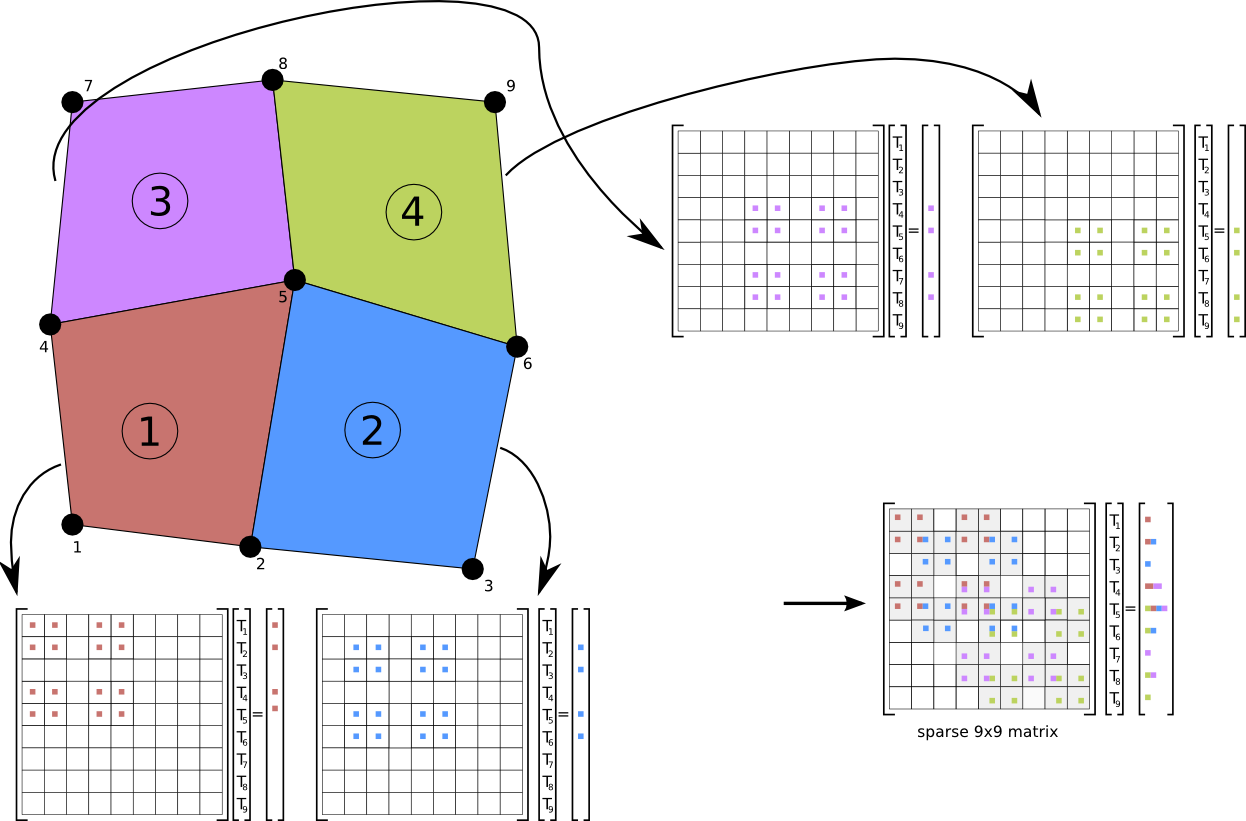
\includegraphics[width=12cm]{images/assembly/assembly.png} 
\end{center}

There are four elements:
\begin{itemize}
\item element 1 is composed of nodes $(1,2,5,4)={\vec T}^{el1}$
\item element 2 is composed of nodes $(2,3,6,5)={\vec T}^{el2}$
\item element 3 is composed of nodes $(4,5,8,7)={\vec T}^{el3}$
\item element 4 is composed of nodes $(5,6,9,8)={\vec T}^{el4}$
\end{itemize}
For each element one has computed an elemental matrix ${\bm A}^{el}$ and a right hand side ${\vec b}^{el}$. 
\[
{\bm A}^{el1} \cdot {\bm T}^{el1} = {\bm b}^{el1}
\]
\[
{\bm A}^{el2} \cdot {\bm T}^{el2} = {\bm b}^{el2}
\]
\[
{\bm A}^{el3} \cdot {\bm T}^{el3} = {\bm b}^{el3}
\]
\[
{\bm A}^{el4} \cdot {\bm T}^{el4} = {\bm b}^{el4}
\]
As seen in the 1D case, these four linear systems must be assembled in a single large matrix of size 
$9\times 9$ as shown in the figure above.

